\documentclass{article}
\usepackage{graphicx}
\usepackage[margin=1in]{geometry}
\usepackage{listings}
\usepackage{amsmath}
\usepackage{minted}

\begin{document}

\title{CS102: Functions}

\maketitle
\section*{Instructions:}
Do problems in order of difficulty, which is indicated by their section placement. Suggested order: 1.1, 2.1, 3.1, 1.2, 2.2, 3.2,  1.3....
\section{Pass By Value}

\subsection{Exponents}
Write, run, and test a C++ function with the following prototype:
\begin{minted}{c++}
	int pow2(int a, int b);
\end{minted}
to find the value of $a^{b}$  by using a for loop, where a and b are integer values that the user enters. And then write a main program to test the function, which is implemented correctly if when the function is called, the following criteria is true:
\begin{minted}{c++}
pow(a,b) == pow2(a,b);
\end{minted}

\subsection{Quadrant}
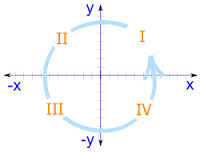
\includegraphics[width=.25\textwidth]{images}\\
Given a cartesian graph (shown above), write a function with the following prototype 
\begin{minted}{c++}
        string quadrant(int x, int y);
\end{minted}
that returns which quadrant the (x,y) point is in, and returns "origin" when x=0 and y=0. And then write a main program to test the function.

\subsection{Coin Toss}
Write a function named coinToss that simulates the tossing of a coin. When you call the function, it should generate a random number in the range of 1 through 2. If the random number is 1, the function should return "heads." If the random number is 2, the function should return "tails." Demonstrate the function in a program that asks the user how many times  the coin should be tossed, and then simulates the tossing of the coin that number of times. 

\subsection{Safest Driving Area}
Write a program that determines which of five geographic regions within a major city (north, south, east, west, and central) had the fewest reported automobile  accidents last year. It should have the following two functions, which are called by main:
\begin{description}
\item[int getNumAccidents] is passed the name of the region and should be called 5 times in total. This function:
		\begin{itemize}
\item asks the user how many accidents were reported in that region during the last year
\item validate the input (no accidents less than 0) and throws an exception on bad input
\item returns the number of accidents for that region
\end{itemize}
\item[void findLowest] is passed the 5 accident totals and their associated regions (so 10 arguments in all). It figures out which region has the lowest total and prints the region and its accident count.
\end{description}
\section{Pass By Reference}
\subsection{Swap}
Write a function that uses the following prototype and swaps the values of the two reference parameters.
\begin{minted}{c++}
	void swap(int &a, int &b);
\end{minted}
 And then write a main to test the function, The function is implemented correctly if after the function is called, b contains the old value of a and a contains the old value of b. For example a and b contain:\\
\begin{tabular}{|l|c|c|}
\hline
& \textbf{a} & \textbf{b}\\
\hline
\textbf{Before function is called} & 2 & 3\\
\hline
\textbf{After function is called} & 3 & 2\\
\hline
\end{tabular}
\subsection{Sort}
Write a function that uses the following prototype to sort a, b, c in ascending order:
\begin{minted}{c++}
void sort(int &a, int &b, int &c);
\end{minted}
And then write a main to test the function, The function is implemented correctly if after the function is called, the following criteria is true: $a<b<c$ For example:

\begin{tabular}{|l|c|c|c|}
\hline
& \textbf{a} & \textbf{b} & \textbf{c}\\
\hline
\textbf{Before function is called} & 4 & 5 & 3\\
\hline
\textbf{After function is called} & 3 & 4 & 5\\
\hline
\end{tabular}

\subsection{Change}
Write a function named \textbf{change} that has an integer parameter and six integer reference parameters named hundreds, fifties, twenties, tens, fives, and ones. The function is to consider the passed integer value as a dollar amount and convert the value into the fewest number of equivalent bills. Using the reference parameters, the function should alter the arguments in the calling function. Then write a program to test that the function is implemented correctly.  

\subsection{Split Decimal Number}
Write a function named \textbf{split} that takes a double parameter and two integer reference parameters named integral and decimal. The function should break up the double parameter into it's integral and decimal parts, and alter the reference parameters accordingly. For example, if the double  parameter is XXX.YYYYY, the function should split up the parameter such that integral=XXX and decimal=YYYY. Then write a program to test that the function is implemented correctly. 

\section{Templates}

\subsection{Display}
\begin{enumerate}
\item Write a function template named display() that displays the value of the single argument passed to it when the function is called.
\item Include the function template in a complete C++ program that calls the function three times: once with a character argument, once with an integer argument, and once with a double precision argument.
\end{enumerate}

\subsection{Whole}
\begin{enumerate}
\item Write a function template named whole() that returns the integer value of any argument passed to it when the function is called.
\item Include the function template  in a complete C++ program that calls the function three times: once with a character argument, once with an integer argument, and once with a double-precision argument.
\end{enumerate}

\subsection{Max}
\begin{enumerate}
\item Write a function template named maximum() that returns the maximum value of three arguments passed to the function when it’s called. Assume that all three arguments are the same data type.
\item Include the function template in a complete C++ program that calls the function with three integers and then with three double-precision numbers.
\end{enumerate}

\subsection{Sort 2}
Modify the sort function from 2.2 so that it sorts three arguments of any type. It should remain a pass-by-reference function. Assume all three arguments are of the same type. Include the function template in a complete C++ program that calls the function with three integers and then with three double-precision numbers. 

\end{document}
